\section{Exécution \& tests} % (fold)
\label{sec:execution}

Pour ce projet, nous avons effectué des tests de validation sur les fonctions algébriques, afin de s'assurer que celles-ci marchaient correctement, et pouvoir plus facilement isoler les problèmes. 
De même, le code a été segmenté pour permettre une lecture plus aisée de l'ordre dans lequel s'effectuent les diverses opérations.

\section{Performances} % (fold)
\label{sec:perf}

Une série de tests est lancée sur différentes tailles de matrice plusieurs fois, afin d'obtenir des temps d'exécution moyens. Nous avons remarqué que pour des matrices de taille croissantes, des erreurs de calcul apparaissaient. Ainsi, pour des matrics de taille $30 \times 30$, les erreurs commençaient à être significatives dans le calcul du dtrsm (de l'ordre de $0.1$).\\
Nous avons remarqué que l'algorithme passait beaucoup de temps dans les fonctions de répartition des données sur les processus. Aussi avons-nous comparé les temps de calculs seulement. \\
La Figure \ref{fig:sp-size} 

\begin{figure}[H]
\centering
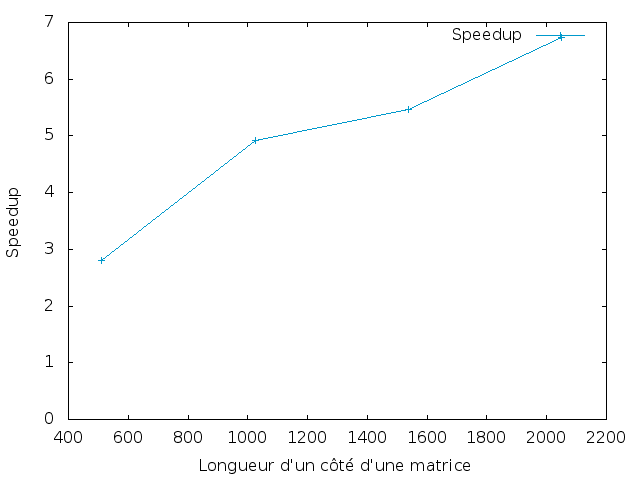
\includegraphics[width=0.8\textwidth]{sp-size.png}
\caption{Accélération de notre programme par rapport au code séquentiel pour une matrice 1024x1024, en fonction du nombre de processeurs}
\label{fig:sp-size}
\end{figure}

Comme l'indique la courbe de la Fig. \ref{fig:sp-proc}, le nombre de processeurs permet de réduire le temps d'exécution. Cette courbe a été tracée sur des matrices de dimensions $1024\times1024$
\begin{figure}[H]
\centering
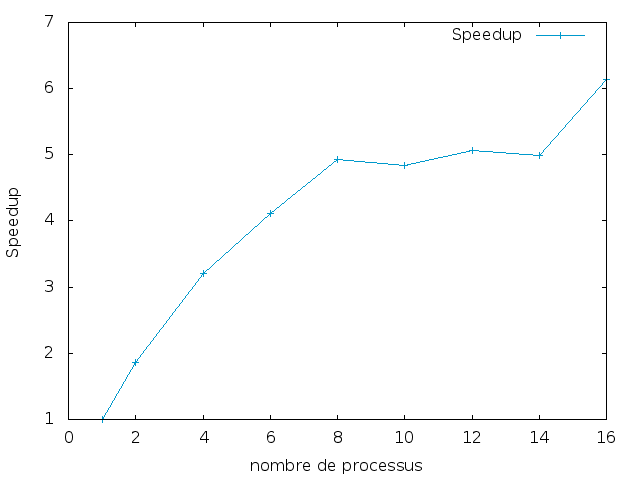
\includegraphics[width=0.8\textwidth]{sp-proc.png}
\caption{Accélération de notre programme par rapport au code séquentiel pour une matrice 1024x1024, en fonction du nombre de processeurs}
\label{fig:sp-proc}
\end{figure}

% section \ (end)
